\chapter{Conclusions}

% This chapter summarises your project, including a concise and significant summary of the R&D project findings, and contributions. 

% Present the outcome, and the arguments.
% Link back to research questions

%\section{Objectives \& Outcomes}


%\section{Research}

The research conducted in this project has identified where the key areas of work are in developing a Digital Twin Platform for Ahuora. 
This has resulted in a framework being proposed for the system, wherein the Digital Twin Platform is built on top of a data processing pipeline and a simulation platform. 
It has been tested via prototyping to show that it is appropriate for those who are involved in both design and operation of the factory, from a data or chemical engineering perspective.

%\section{Development}

This has been implemented in the Ahuora Digital Twin Platform for steady-state modelling. 
The ability to store solve history was added to visualise the results of simulations, and functionality to preprocess data was added to make it possible to convert input data to the format required in chemical modelling. 

As a test case, a model of a heat pump dryer was created and the platform was used to simulate the dryer's performance. 
This showed that the platform is capable of simulating a factory's performance, and identified some edge cases where care must be taken to specify the model in a way that it can be reliabily solved.

%\section{Future Work}
% Strengths, limitations, impacts, what could have been better, etc


\section{Future work}
% TODO: Update this section from the interlude
Future work could focus on adding support for dynamic models, hybrid modelling, and optimisation to the Ahuora Platform. Then the live data processing system could be developed to support these features. 
This would increase the usefulness of the platform for factory operation and control. 


The research conducted so far has provided the context required to build a high-level roadmap of future development. This is shown in \Cref{fig:development_flowchart}, where the development is broken down into phases. Each phase is broken down into subtasks, identifiying the key challenges to overcome.
Phase 1 provides the core functionality: ingesting data, solving the simulation, and displaying the results. This is the minimum viable product, and constitutes the main objective of this project. Phase 2 adds support for physics based modelling, optimisation, and control. The key challenges anticipated, including specifying input of the the time domain, holdup, and visualisation, come from the research conducted in \Cref{sec:dynamicmodelling}. Likewise, the key challenges from optimisation and control originate from the research in \Cref{sec:optimisationcontrol}. Based on research from the literature review and \Cref{sec:surrogatemodelling} surrogate modelling moves beyond IDAES alone, and may also include online learning methods, specified in the figure as ``Live Surrogate Modelling''. This was seperated out as Phase 3, because it is a wider goal, and less defined at this stage. 

Phase 2 and 3 will not be developed in this project, but the long-term roadmap is a key research outcome in itself. This proves that development has been done in an engineering context, with a clear understanding of future requirements and an anticipation of further work.

% Todo: Put this in the appendix
\begin{landscape}
    \begin{figure}
        \centering
        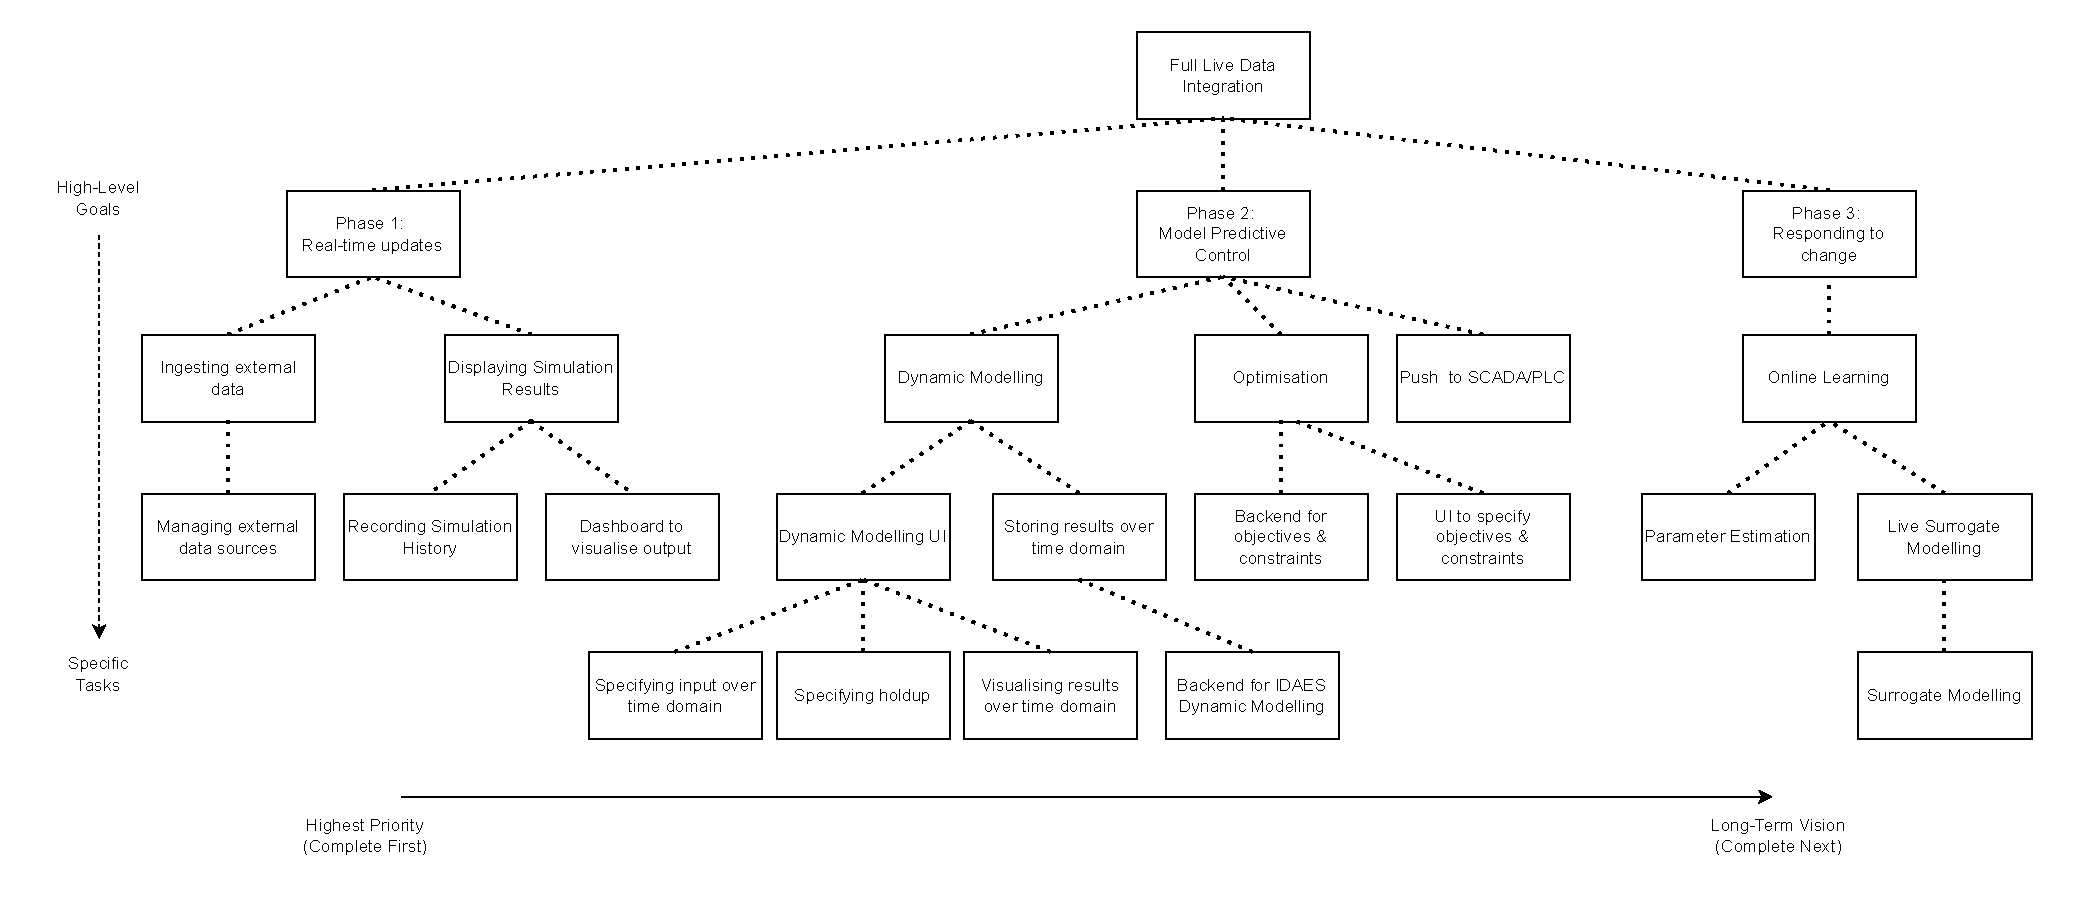
\includegraphics[width=1.5\textwidth]{roadmap.pdf}
        \caption{Roadmap of future development, broken down into tasks. This extends beyond the scope of this project, into the broader vision of the Ahuora Digital Twin Platform. Each task is a key milestone in creating an industry-ready live data processing platform.}
        \label{fig:development_flowchart}
    \end{figure}
\end{landscape}

A standalone `Deployment' version of the Ahuora Platform, specifically focused on control and optimisation, could also be created. 
This could better fit the constraints of a real factory, where cloud platforms may not be appropriate.

%\section{Impact Statement}

This work addressed some of the main challenges in implementing digital twins in the industry, namely, the complexity and cost of building a Digital Twin system from scratch. Through the continued development of Digital Twin Platforms as specified in this report, Project Ahuora's goal to decarbonise the process heat sector will be fully realised.
% evaluates the broader impact of the project outcome, either quantitatively or qualitatively (e.g., social, economic, environmental, health, safety, legal, ethical, and/or cultural issues)
%\section{Impact}


